% small.tex
\documentclass{beamer}
\usetheme{Madrid}
%Berlin(bottom bar) / Frankfurt (more room) / Copenhagen (more room, bottom bar|split)
\usepackage[orientation=landscape, size = a0, scale=1.4]{beamerposter}
\usepackage[relative,overlay]{textpos}
\usepackage{graphicx}
\usepackage{wrapfig}
%algorithms and pseudo code
\usepackage{algorithm}
\usepackage[noend]{algpseudocode}
\usepackage{numprint}
\usepackage{subcaption}
\usepackage{media9}
\usepackage{bibentry}
\usepackage[justification=centering]{caption}
\usepackage{pagecolor}
\usepackage{background}
\usepackage{blindtext}
\usepackage{color}
\usepackage{xcolor}
\usepackage{enumitem}
\usepackage{ragged2e}
\setlist[itemize,1]{label=\textbullet}
\setlist[itemize,2]{label=*}
\usepackage{caption}
\captionsetup[figure]{labelformat=empty}

\nobibliography*

\renewcommand\familydefault{cmss}
\newcommand\Xlft{5mm} \newcommand\Xrt{836mm}
\newcommand\Ytop{5mm} \newcommand\Ybtm{1164mm}
\newcommand\PaneW{390mm}
\definecolor{navyblue}{RGB}{0,0,128}
\font\footerfont=cmr12 at 45pt
\makeatletter
\setbeamertemplate{footline}
{
  \leavevmode%
  \hbox{%
  \begin{beamercolorbox}[wd=\paperwidth,ht=7ex,dp=3.5ex,center]{author in head/foot}%
    \footerfont {\bf Contact:} Gerrett Diamond (\underline{diamog@rpi.edu}), Cameron Smith (\underline{smithc11@rpi.edu}), and Mark Shephard (\underline{shephard@rpi.edu})
  \end{beamercolorbox}%
  \begin{beamercolorbox}[wd=.333333\paperwidth,ht=4ex,dp=1ex,center]{title in head/foot}%
    \usebeamerfont{title in head/foot}Contact:
  \end{beamercolorbox}%
  \begin{beamercolorbox}[wd=.333333\paperwidth,ht=4ex,dp=1ex,right]{date in head/foot}%
    \usebeamerfont{date in head/foot}\insertshortdate{}\hspace*{2em}
%    \insertframenumber{} / \inserttotalframenumber\hspace*{2ex} % DELETED
  \end{beamercolorbox}}%
  \vskip0pt%
}
\makeatother
%\setbeamertemplate{bibliography item}[text]
%\setbeamertemplate{author in head/foot}{\insertshortauthor}
%\setbeamertemplate{navigation symbols}{}

\newcommand{\lenitem}[2][.6\linewidth]{\parbox[t]{#1}{\strut #2\strut}}

\setbeamercolor{background canvas}{bg=cyan!50}
\setbeamercolor{block title}{bg=navyblue!80}
\setbeamercolor{block body}{bg=white,fg=black}
\begin{document}
\title[]
{\bf \fontsize{100}{110}\selectfont
Diffusive Load Balancing for Relation-Based Data
}
\author[]{\fontsize{50}{60}\selectfont
  Gerrett Diamond, Cameron W. Smith, Mark S. Shephard\\
  Rensselaer Polytechnic Institute, USA}
\date{}
\begin{textblock}{15.6}(0,0)
  \titlepage
  \begin{textblock}{14.5}(.75,-0.65)
    \setbeamercolor{block body}{bg=navyblue!80,fg=white}
    \begin{block}{}
      \begin{textblock}{14}(0.25,0.1)
        \centering
        \justify
          \fontsize{37}{43}\selectfont
      Parallel applications with complicated data structures and communicative patterns
      require partitioning algorithms that optimize specific metrics. While most
      partitioning methods can create partitions of a decent quality, further
      optimizations can be made for applications using diffusive load balancing techniques.
      EnGPar complements existing multi-level and geometric partitioning methods by supporting
      multi-criteria partition improvement. EnGPar utilizes a specialized multi-graph, called
      the N-graph, to represent relation based data in order to perform load balancing for a
      range of data formats.
      \end{textblock}
      \vspace{5cm}
    \end{block}
  \end{textblock}
\end{textblock}
\begin{textblock}{4}(0,.7)
  \begin{figure}
    
\includegraphics[width=\textwidth]{../logos/RPI.png}
  \end{figure}

\end{textblock}
\begin{textblock}{2}(13.6,.6)
  \begin{figure}
    
\includegraphics[width=\textwidth]{../logos/SCOREC_backgroundless.png}
  \end{figure}

\end{textblock}

\begin{textblock}{15.6}(0,2.9)
  \begin{textblock}{5.1}(0,0)
    \begin{block}{\centering Partitioning of Relation-based Data}
      Many parallel applications running on current and next generation systems utilize some form of relational data that must be partitioned to achieve optimal runtime performance including:
      \begin{itemize}
      \item Graphs/scale-free graphs, structured/unstructured meshes, and matrices.
      \end{itemize}
      Common methods applied to partition these structures are:
      \begin{itemize}
      \item Graph, hypergraph, and geometric.
      \end{itemize}
      However these methods are not always sufficient for an application to achieve optimal performance. \\Examples will show common applications that require more specific load balancing and how our system can be used to target each.
    \end{block}
    \begin{block}{\centering EnGPar: Diffusive Graph Partitioning}
      The N-graph is defined as the following:
      \begin{itemize}
      \item Set of vertices $V$ representing atomic units of work.
      \item For the traditional graph mode:
        \begin{itemize}
        \item $N$ sets of edges $E_0,...,E_{n-1}$ for each relation type.
        \item Edges connect two vertices $u,v \in V$.
        \end{itemize}
      \item For the hypergraph mode:
        \begin{itemize}
        \item $N$ sets of hyperedges $H_0,...,H_{n-1}$ for each relation type.
        \item $N$ sets of pins $P_0,...,P_{n-1}$ for each hyperedge set.
        \item Each pin in $P_i$ connects vertex, $v \in V$, to hyperedge $h \in H_i$.
        \end{itemize}
      \end{itemize}

      Advantages
      \begin{itemize}
      \item Multiple edge types allow partitioning for multiple criteria.
      \item Integrates with partitioning tools to create initial partitions.
      \item Compliments partition methods via incremental refinements.
      \end{itemize}
      
      Diffusive Approach
      \begin{itemize}
      \item Iteratively migrate small sets of vertices to \\(1) reduce peak imbalance \\(2) reduce number of (hyper)edges cut between part boundaries.
      \end{itemize}
    \end{block}
    \begin{block}{\centering Supporting Accelerators}
      \begin{itemize}
      \item EnGPar is designed to support many-core processors and accelerators (GPU, FGPA).
      \item OpenCL implementation of BFS is 7x faster on GPU than serial CPU (including data copy).
      \item Working on data (GPU) and pipeline (FPGA) parallel kernels of other diffusive procedures.
      \end{itemize}

    \end{block}
    \begin{block}{\centering More Information}
      EnGPar: \url{http://scorec.github.io/EnGPar/} \\
      SCOREC: \url{https://www.scorec.rpi.edu/}
    \end{block}

  \end{textblock}
  \begin{textblock}{5.1}(5.25,0)
    \begin{block}{\centering Finite Element Analysis: Unstructured Meshes}
      %FEM description
      Applications using unstructured meshes exhibit several partitioning problems:
      \begin{itemize}
      \item Multiple coupled entity dimensions to partition.
      \item Complex communication patterns to be minimized.
      \end{itemize}
      
      %N-graph construction
      \begin{textblock}{3.2}(0,0.1)
        To achieve the best performance, FEA problems require:
        \begin{itemize}
        \item Mesh entities holding dof to be balanced,
        \item Mesh elements to be balanced.
        \end{itemize}
        To properly balance, we construct the N-graph where:
        \begin{itemize}
        \item Mesh elements are represented as graph vertices,
        \item Mesh entities holding dof are represented by hyperedges, and
        \item Pins are created from graph vertex to hyperedge where the mesh element is bounded by the mesh vertex.
        \end{itemize}
      \end{textblock}
      \begin{textblock}{2.5}(2.7,-.7)
      \begin{figure}
        \centering
        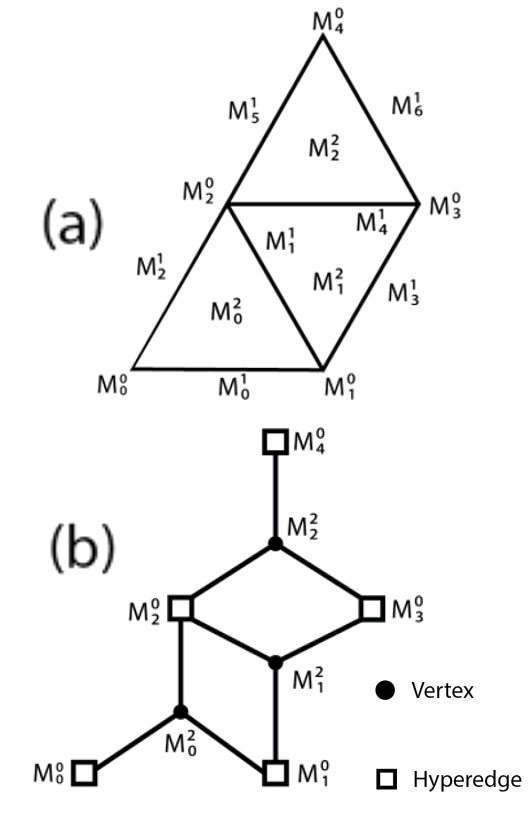
\includegraphics[width=.75\textwidth]{../figures/mesh2Graph_vert.png}
        \caption{Conversion from mesh (a) to N-graph (b)}
      \end{figure}
      \end{textblock}
      \vspace{20cm}
    \end{block}
    \begin{block}{\centering Strong Scaling on an Unstructured Mesh}
      %Discuss testing
      Tests were run on a one billion element mesh created and partitioned using:
      \begin{itemize}
      \item Global ParMETIS part k-way to 8Ki($8*2^{10}$) parts and
      \item Local ParMETIS part k-way from 8Ki to 128Ki, 256Ki, and 512Ki parts.
      \end{itemize}
      \begin{textblock}{2.5}(2.4,.25)
        \begin {itemize}
        \item Creating the 512Ki partition from 8Ki parts takes 147 seconds with ParMETIS (includes migration). 
        \item EnGPar reduces a 53\% vtx imbalance to 13\% in 7 seconds on 512Ki processes. 
        \end{itemize}
      \end{textblock}
      \begin{textblock}{2.5}(0,0)
      \begin{figure}
        \centering
        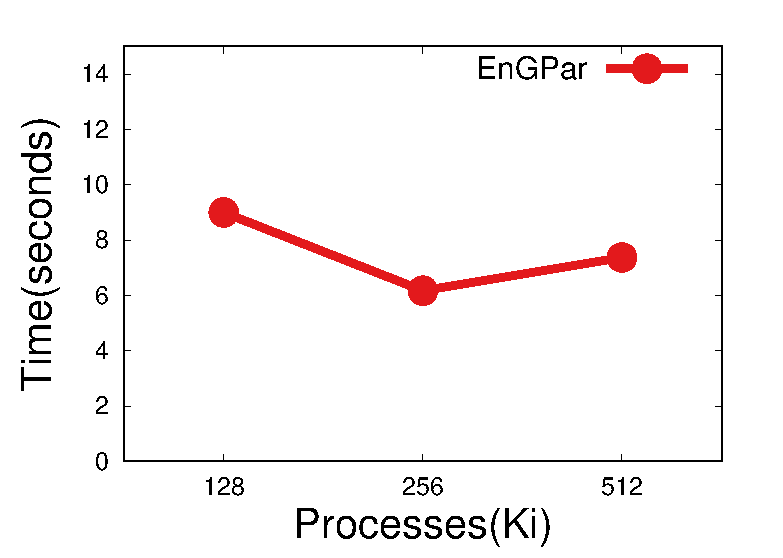
\includegraphics[width=.9\textwidth]{../plots/mira_fem_results/time_v_cores.eps}
      \end{figure}
      \end{textblock}
      \vspace{11.5cm}
      
      \begin{figure}
        \centering
        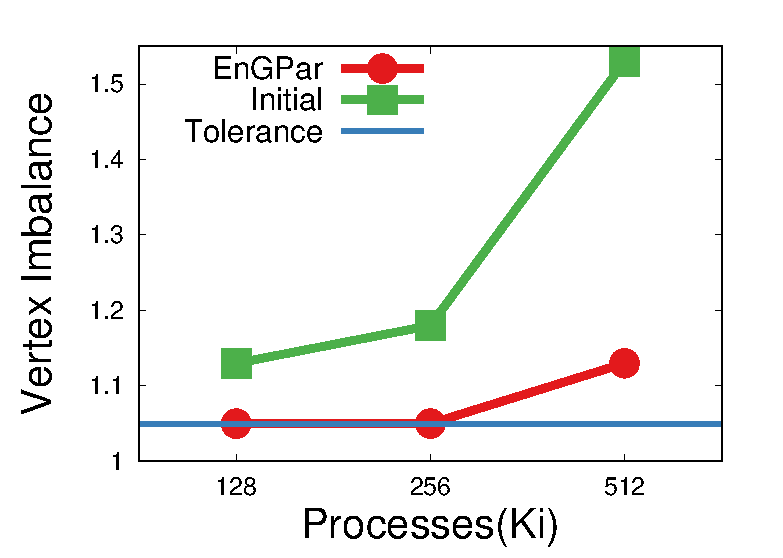
\includegraphics[width=.45\textwidth]{../plots/mira_fem_results/vimb_v_cores.eps}
        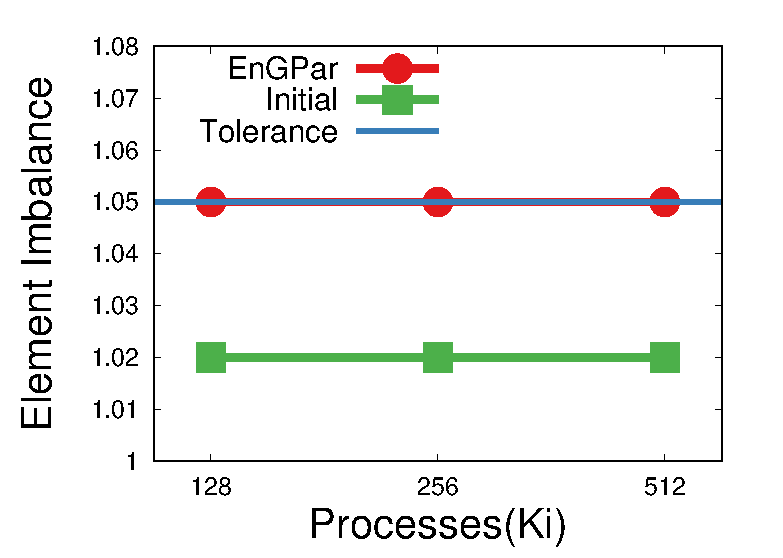
\includegraphics[width=.45\textwidth]{../plots/mira_fem_results/eimb_v_cores.eps}
        \caption{Resulting imbalances after running EnGPar}
      \end{figure}
    \end{block}

    \begin{block}{\centering Acknowledgement}
      \begin{textblock}{3.5}(0,0)
      \begin{itemize}
      \item National Science Foundation Grant ACI 1533581
      \item DOE FASTMath SciDAC Institute
      \item CEED ECP Co-Design Center
      \end{itemize}
      \end{textblock}
      \begin{textblock}{1.5}(3.5,0)
        \begin{itemize}
          \item DoD PETTT program
        \end{itemize}
      \end{textblock}
      \vspace{4.2cm}
    \end{block}
  \end{textblock}
  \begin{textblock}{5.2}(10.5,0)
    \begin{block}{\centering General Partitioning}
      To further explore the capabilities of EnGPar, we are looking at several applications beyond the standard FEA example including:
      \begin{textblock}{2.5}(0,0.05)
        \begin{itemize}
        \item Overset grids 
        \end{itemize}
      \end{textblock}
      \begin{textblock}{2.5}(1.3,0.05)
        \begin{itemize}
        \item Particle meshes
        \end{itemize}
      \end{textblock}
      \begin{textblock}{2.5}(2.6,0.05)
        \begin{itemize}
        \item Discrete Event Simultations
        \end{itemize}
      \end{textblock}
      \vspace{1.6cm}
    \end{block}
    \begin{block}{\centering CODES: Discrete Event Simulations}
      \begin{textblock}{3.3}(0,0)
      CODES simulates running an MPI application on a simulated
      hardware architecture. The main unit of CODES is logical processes (LPs) which are used
      to represent the hardware components and simulated MPI processes. \\[.2cm]
      The N-graph construction includes:
      \begin{itemize}
      \item Graph vertices are created for each LP.
      \item Graph edges are added between LPs that have an event between them.
      \end{itemize}

      \end{textblock}
      \begin{textblock}{2}(3.3,-.15)
        \begin{figure}
          \centering
          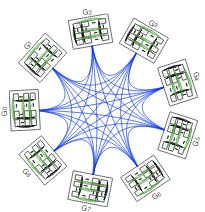
\includegraphics[width=.8\textwidth]{../figures/dragonfly.png}
          \caption{A dragonfly network [1]}
        \end{figure}
      \end{textblock}
      \vspace{13.6cm}
    \end{block}
    \vspace{-.7cm}
    {\fontsize{22}{23}\selectfont 1 - Trade-off Study of Localizing Communication and Balancing Network Traffic on Dragonfly Systems X. Wang et al. 2018
    }
    \begin{block}{\centering Overset Grids}
      Some unstructured mesh applications are accompanied with an overset grid.
      \begin{textblock}{3}(0,0.1)
        %More info about the overset grid applications
        These simulations add additional partitioning challenges such as:
        \begin{itemize}
        \item Computational coupling between meshes
        \item Additional communication/part boundaries
        \end{itemize}
        N-graph construction includes:

      \end{textblock}
      \begin{textblock}{2.5}(2.7,0)
        %example image of the overset grid + mesh
        \begin{figure}
          \centering
          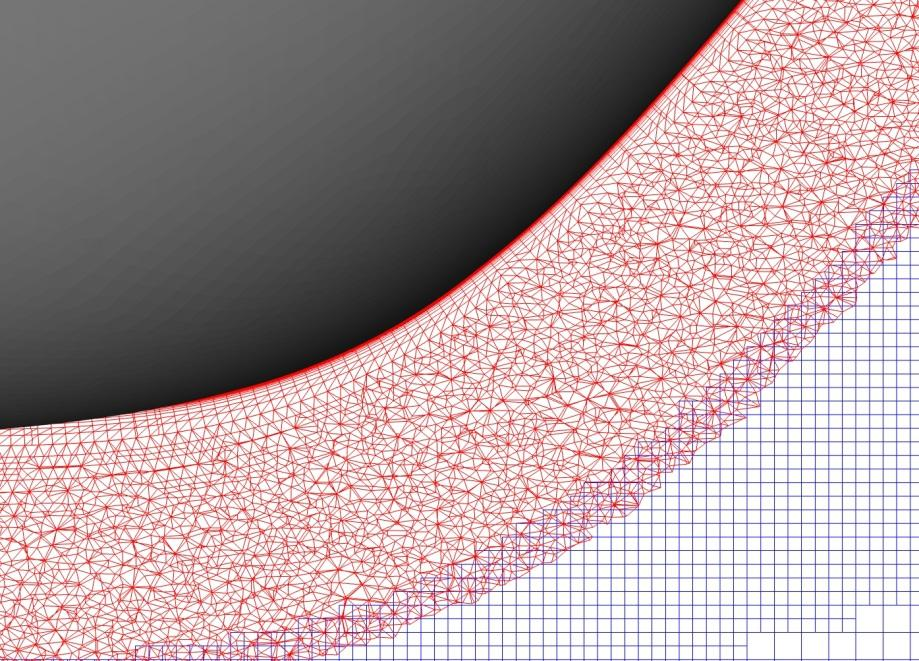
\includegraphics[height=.5\textwidth]{../figures/overset_grid.jpg}
          \caption{An unstructured mesh (in red) with \\overset grid (in black) [2].}
        \end{figure}
      \end{textblock}
      \vspace{9.1cm}

      
      %Describe the construction of the N-graph
      \begin{itemize}
      \item Vertices for elements in the overset grid.
      \item Vertices/edges on unstructured mesh.
      \item Second edge type connects graph vertices where mesh/grid overlap.
      \end{itemize}
      
    \end{block}
    
    \begin{block}{\centering FUN3D: Fluid dynamics simulations}
      A finite-volume application that has partitioning requirements:
      \begin{textblock}{3.5}(0,0.1)
      \begin{itemize}
      \item Vertex partitioned nonconforming mesh.
      \item A ghost layer at part boundaries.
      \item An overset grid for other simulations.
      \end{itemize}
      \end{textblock}
      \begin{textblock}{2.5}(2.9,-0.05)
        \begin{figure}
          \centering
          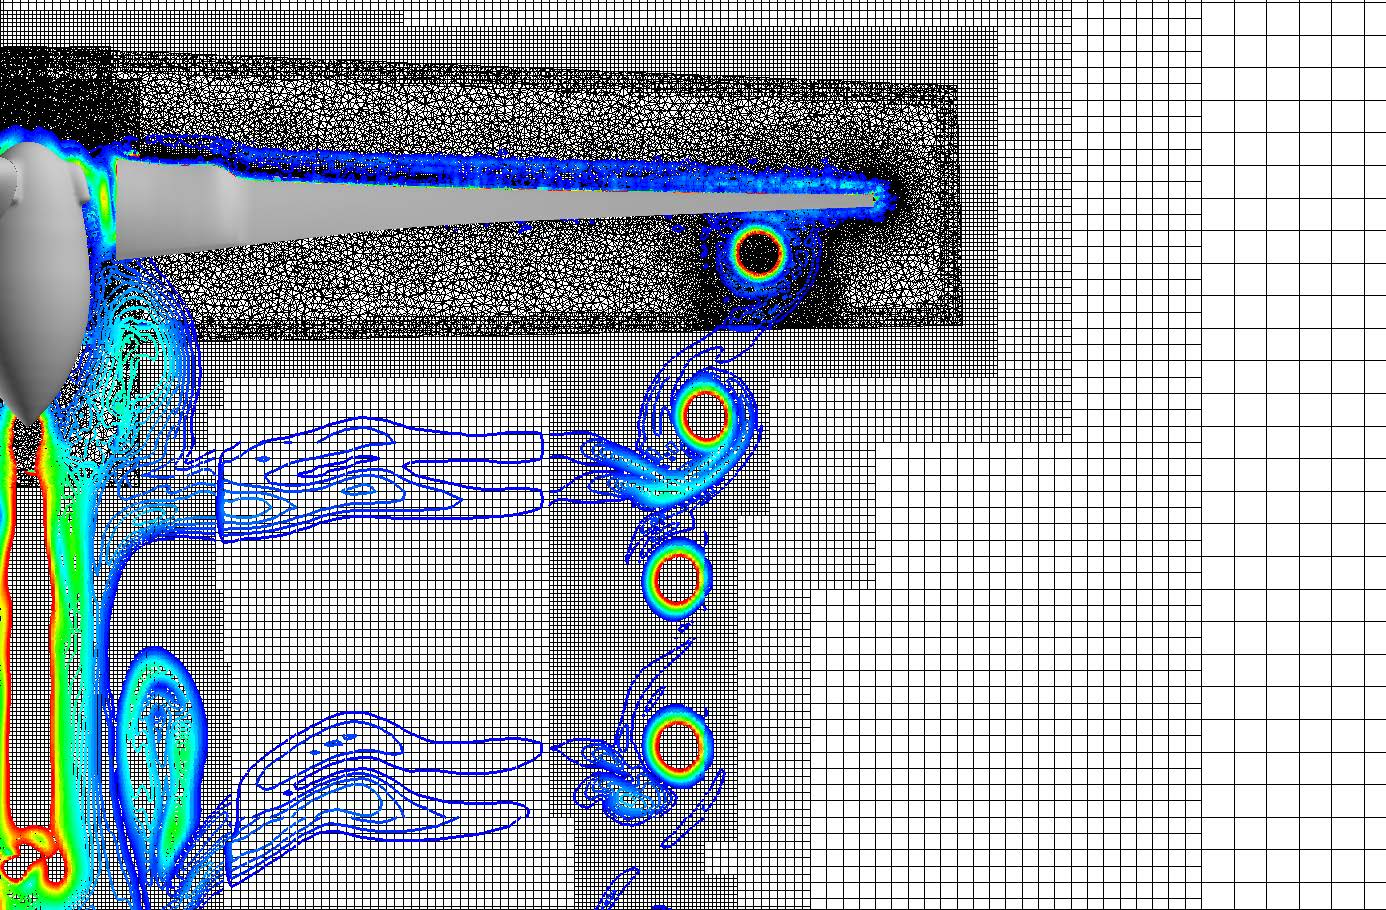
\includegraphics[width=.8\textwidth]{../figures/FUN3D.jpg}
          \caption{Airflow solution of a plane[2].} 
        \end{figure}
      \end{textblock}
      \vspace{5.25cm}
      %Discuss construction of N-graph
      N-Graph construction includes:
      \begin{itemize}
      \item Graph vertices from mesh vertices
      \item Hyperedges for each mesh element
      \item Pins between mesh elements and mesh vertex.
      \item Ghosted vertices are weighted during diffusive iterations.
      \item The overset grid is accounted for similar to above.
      \end{itemize}
      
    \end{block}
    \vspace{-.7cm}
    {\fontsize{22}{23}\selectfont 2 - "Progress in Strand/Cartesian Overset CFD simulations using CREATE™-AV Helios" J. Sitaraman et al. 2017
    }

    \begin{block}{\centering Closing Remarks}
      EnGPar utilizes diffusive methods to improve the partition of distributed data. \\
      Furthemore, EnGPar's generalized graph structure allows for the techniques to \\
      multiple applications.
    \end{block}
  \end{textblock}
\end{textblock}

\end{document}
